\section{Evaluation}
\label{sec:eval}

\begin{figure*}
    \centering
    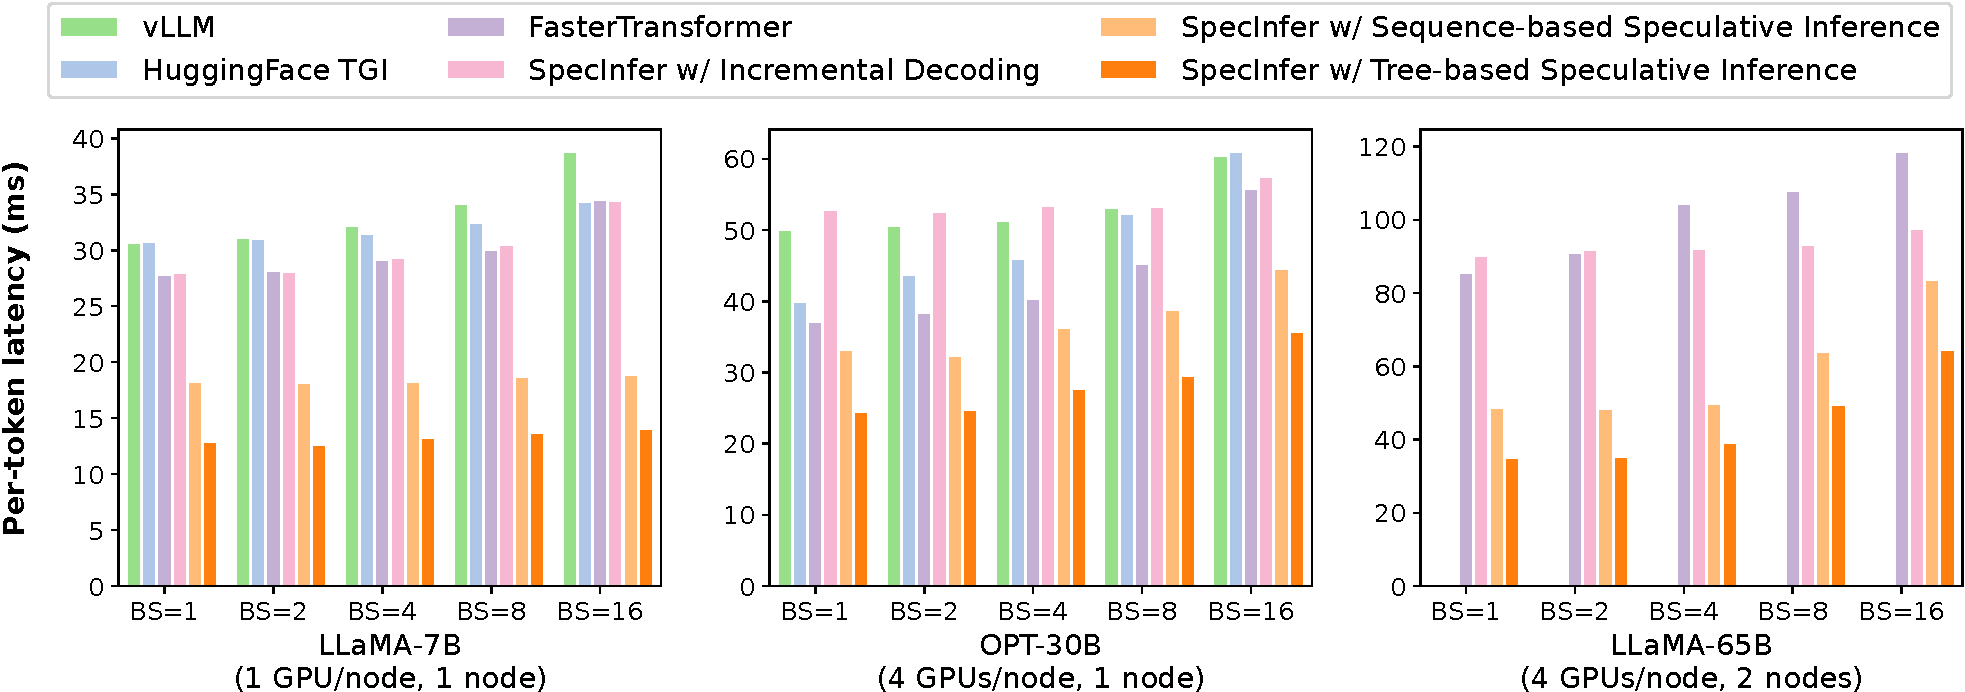
\includegraphics[scale=0.52]{figs/revised_end_to_end2-crop.pdf}
    \caption{\rev{Comparing the end-to-end inference latency of \Sys with existing systems. Numbers in parenthesis show the number of GPUs and compute node used to serve each LLM. All systems parallelize LLM inference by combining tensor model parallelism (within a node) and pipeline parallelism (across nodes).}
    %We use \llama-7B as the LLM and all SSMs are derived from \llama-68M.
    %The performance is normalized by incremental decoding, and the numbers on the \Sys bars indicate the speedups over incremental decoding.
    }
    \label{fig:latency}
\end{figure*}

\subsection{Experimental Setup}
\label{subsec:setup}

\paragraph{LLMs.} To compare the runtime performance of \Sys with existing LLM serving systems, we evaluate these systems using two publicly available LLM families: OPT~\cite{zhang2022opt} and \llama~\cite{touvron2023llama}. 
%%%
More specifically, we select \llama-7B, OPT-13B, OPT-30B, and \llama-65B as the LLMs, and \llama-68M and OPT-125M as the SSMs.
%%%
%\Cref{sec:cbt_method} describes how \Sys collectively boost-tunes multiple SSMs from the pre-trained one.
The pre-trained model parameters for the LLMs and SSMs were obtained from their HuggingFace repositories~\cite{huggingface}, and we describe how \Sys collectively boost-tunes multiple SSMs in~\cite{miao2023specinfer}.
% \Cref{sec:cbt_method}.
%%%
%\Cref{subsec:eval_boost_tuning} evaluates how collective boost-tuning can further improve speculation performance.

\paragraph{Datasets.} We evaluate \Sys on five datasets: Chatbot Instruction Prompts (CIP)~\cite{chatbot2023}, ChatGPT Prompts (CP)~\cite{mohamed2023chatgpt}, WebQA~\cite{berant-etal-2013-semantic}, Alpaca~\cite{alpaca, peng2023instruction}, and PIQA~\cite{Bisk2020}. 
%%%
We only use the prompts/questions from these datasets to form our input prompts to simulate real-world conversation traces.
%%%
%We randomly selected at most 1000 prompts from each dataset in our evaluation.


\paragraph{Platform.} The experiments were conducted on two AWS {\tt g5.12xlarge} instances, each of which is equipped with four NVIDIA A10 24GB GPUs, 48 CPU cores, and 192 GB DRAM. Nodes are connected by 100 Gbps Ethernet.
%\Sys serves OPT-30B and \llama-30B in half-precision floating points across four A10 GPUs using tensor model parallelism.
%OPT-66B and \llama-65B do not fit on four A10 GPUs, therefore \Sys serves these two LLMs on eight A10 GPUs across two compute nodes.
%The LLMs used in our evaluation do not fit on a single T4 GPU. 
%Therefore \Sys performs LLM inference in single-precision floating points and serves the LLMs across the four GPUs using pipeline model parallelism.
%%%
%\Sys serves each SSM on a dedicated GPU and runs these SSMs in parallel for a given sequence of tokens.

Our experiments use the expansion-based method (see \Cref{sec:speculation}) for constructing token trees and use the expansion configuration $\langle 1, 1, 3, 1, 1, 1, 1, 1\rangle$, which provides good results for our benchmarks. We analyze the impact of expansion configurations in \S\ref{subsec:eval_token_tree}, evaluate tree-based parallel decoding and multi-step speculative sampling in \S\ref{subsec:eval_tree_based_decoding} and \S\ref{subsec:eval_msss}, and finally compares the expansion- and merge-based tree construction methods in~\cite{miao2023specinfer}.
% \Cref{sec:eval_tree_construction_methods}.

%\Cref{subsec:eval_token_tree} evaluates the impact of different tree construction methods.
%For all experiments in \Cref{subsec:eval_distributed} and \Cref{subsec:eval_offload}, \Sys uses two SSMs and a speculation depth of 8, which achieves good performance in practice. \XM{\Cref{subsec:eval_boost_tuning}} evaluates how different numbers of SSMs affect \Sys's performance.

\subsection{Distributed LLM Inference}
\label{subsec:eval_distributed}
We compare the end-to-end distributed LLM inference performance among \Sys, vLLM~\cite{vllm}, HuggingFace Text Generation Inference (TGI)~\cite{huggingface_tgi}, and FasterTransformer~\cite{fastertransformer} on \llama-7B, OPT-30B, and \llama-65B.
For \llama-7B and OPT-30B, all systems serve the two LLMs in half-precision floating points across one and four A10 GPUs using tensor model parallelism.
\llama-65B do not fit on four GPUs on a single node, therefore both FasterTransformer and \Sys serve it on eight A10 GPUs on two nodes by combining tensor model parallelism within each node and pipeline model parallelism across nodes.
%%%
vLLM and HuggingFace TGI do not support pipeline model parallelism and cannot serve an LLM on multiple nodes.

To rule out potential effects of our system implementation, we also evaluate \Sys with two additional configurations. First, \sys with {\em incremental decoding} evaluates the runtime performance of our implementation when the speculator generates empty token trees, and the verifier verifies exactly one token in each decoding step.
Second, \sys with {\em sequence-based speculative inference} serves as a reference for existing speculative inference system and is enabled by using a single pre-trained SSM and sequence-based decoding.

We use prompts from the five datasets described in \S\ref{subsec:setup}. For each prompt, we let all systems generate up to 128 new tokens and report the average per-token latency in \Cref{fig:latency}.
%%%
Note that \Sys may generate more than 128 new tokens since the verifier can verify multiple tokens in each iteration. 
In this case, we truncate \Sys's output to 128 tokens.
\Sys with incremental decoding achieves on-par performance as existing  systems. This is because all systems use the same strategies to parallelize LLM inference across GPUs and use the same kernel libraries (i.e., cuDNN, cuBLAS, and cuTLASS) to execute inference computation on GPUs.
%%%
With tree-based speculative inference and verification, \Sys outperforms incremental decoding systems by 1.5-2.5$\times$ for single-node, multi-GPU inference and by 2.4-2.8$\times$ for multi-node, multi-GPU inference, while generating the exact same sequence of tokens as incremental decoding for all prompts.
%%%
\rev{The speedup comes from leveraging spare GPU resources to perform tree-based parallel decoding while maintaining the same per-iteration latency as incremental decoding.}
%The performance improvement is realized by \Sys's ability to verify multiple tokens in a single LLM decoding step.

\rev{Compared to sequence-based speculative inference, \sys's tree-based approach further reduces LLM serving latency by 1.2-1.5$\times$. The improvement is achieved by (1) leveraging token trees to optimize speculative performance, (2) using tree-based parallel decoding to verify an entire token tree in parallel, and (3) performing multi-step speculative sampling to improve verification performance. We further evaluates these aspects in \S\ref{subsec:eval_token_tree}, \S\ref{subsec:eval_tree_based_decoding}, and \S\ref{subsec:eval_msss}.}


\iffinal
Note that \sys's performance improvement over existing systems reduces as the batch size (i.e., number of concurrent requests) increases.
%%%
This is because \sys leverages spare GPU resources to perform tree-based parallel decoding while maintaining the same per-iteration latency as incremental decoding.
%%%
A larger batch size introduces more parallelizable computation for incremental decoding, and thus less spare GPU resources that can be leveraged by \sys.
On the flip side, larger batch sizes also increase the end-to-end latency of each request, as shown in \Cref{fig:latency}.
%%%
Overall, \sys is most beneficial for {\em low-latency} LLM inference.
\fi 

%We compare the end-to-end inference latency between incremental decoding and \Sys on the five prompt datasets. For each prompt dataset, we measured the inference latency of the two approaches on up to 1000 prompts and reported the average inference latency. \Cref{fig:latency} shows the results. Compared to incremental decoding, \Sys reduces the inference latency by 1.9 - 2.7$\times$ while generating the exact same sequence of tokens as incremental decoding for all prompts. The performance improvement is mostly realized by \Sys's ability to verify multiple tokens in a single LLM decoding step.
%%%
%Next, we evaluate how collective boost-tuning and the learning-based speculative scheduler help improve \Sys's inference performance.

\subsection{Offloading-based LLM Inference}
\label{subsec:eval_offload}
\begin{figure}
    \centering
    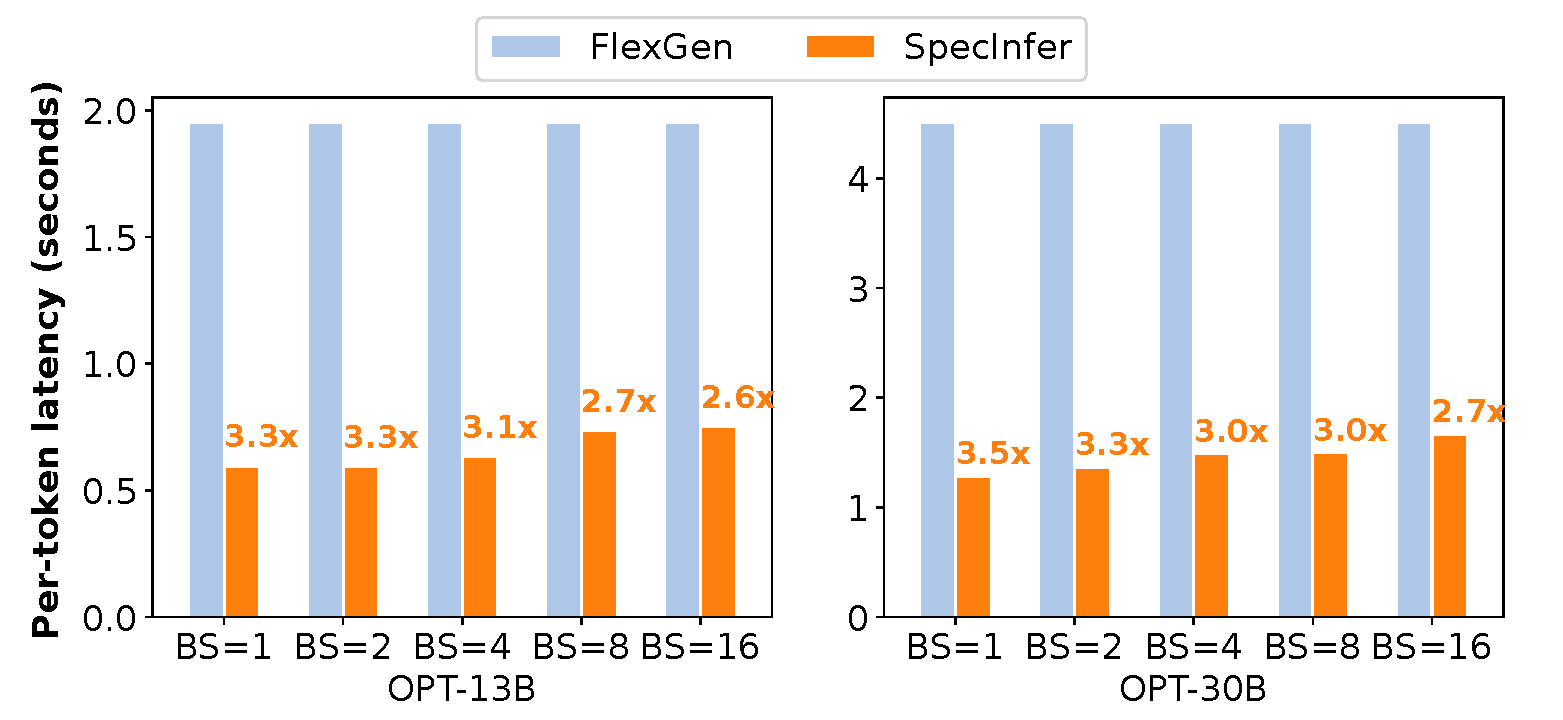
\includegraphics[scale=0.33]{figs/end_to_end_offload2.pdf}
    \caption{Comparing the end-to-end offloading-based inference latency of FlexGen and \Sys. Both FlexGen and \Sys perform model offloading to serve OPT-13B and OPT-30B models on a single 24GB A10 GPU.}
    %\vspace{-4mm}
    \label{fig:eval_offload}
\end{figure}

Another important application of \Sys is offloading-based LLM inference, where the system offloads an LLM's parameters to CPU DRAM and loads a subset of these parameters to GPUs for inference computation in a pipeline fashion.
%%%
We compare the end-to-end offloading-based LLM inference performance between \Sys and FlexGen~\cite{sheng2023flexgen} using a single 24GB A10 GPU and two LLMs (i.e., OPT-13B and OPT-30B), both of which exceed the memory capacity of an A10 GPU and requires offloading for serving. Both \Sys and FlexGen retain all model parameters on CPU DRAM. During computation, the demand weights are loaded from the CPU to the GPU.
%%%
\Cref{fig:eval_offload} shows the results. Compared to FlexGen, \Sys reduces the per-token latency by 2.6-3.5$\times$. 
%%%
Since offloading-based LLM inference is mostly bottlenecked by the communication between CPU DRAM and GPU HBM for loading an LLM's parameters, \Sys's improvement over existing systems is achieved by opportunistically verifying multiple tokens, which in turn reduces the number of LLM decoding steps and data transfers between CPU and GPU.

\subsection{\rev{Token Tree Construction}}
\label{subsec:eval_token_tree}

% \begin{figure}
%     \centering
%     %\subfloat[Greedy sampling CDF.]{
%     %\includegraphics[width=0.33\linewidth]{figs/Greedy sampling CDF.pdf}
%     %}
%     \subfloat[Greedy sampling \textcolor{blue}{This is the CDF figure of greedy decoding}.]{
%     \includegraphics[width=0.5\linewidth]{figs/Greedy decoding CDF.pdf}
%     }
%     \subfloat[Stochastic sampling.]{
%     \includegraphics[width=0.5\linewidth]{figs/Stochastic sampling CDF.pdf}
%     }
%     \caption{CDF figures of greedy sampling, stochastic sampling and greedy decoding. \ZJ{TODO: (1) increase font size for the y-axis title; (2) change the title to ``Average \# verified tokens per decoding step''; (3) add a ``='' between tree width and value}
%     }
%     \label{fig:ssms_greedy_coding}
% \end{figure}



\rev{This section evaluates the expansion-based token tree construction mechanism. We first study how token tree width affects \Sys's speculative performance. In this experiment, we use \llama-7B and \llama-68M as the LLM and SSM, and use the expansion configuration $\langle 1, 1, k, 1, 1, 1, 1, 1\rangle$ (i.e., expanding at the third token), where $k$ is the token tree width.
\Cref{fig:eval_cdf} shows the cumulative distribution function (CDF) of the average number of verified tokens per decoding step for all prompts in the Alpaca dataset~\cite{alpaca}.
%
Compared to sequence-based speculation (i.e., tree width = 1), leveraging token trees can reduce LLM decoding steps by 1.2-1.5$\times$ for greedy decoding and by 1.3-1.4$\times$ for stochastic decoding.}

\begin{figure}
    \centering
    %\subfloat[Greedy sampling CDF.]{
    %\includegraphics[width=0.33\linewidth]{figs/Greedy sampling CDF.pdf}
    %}
    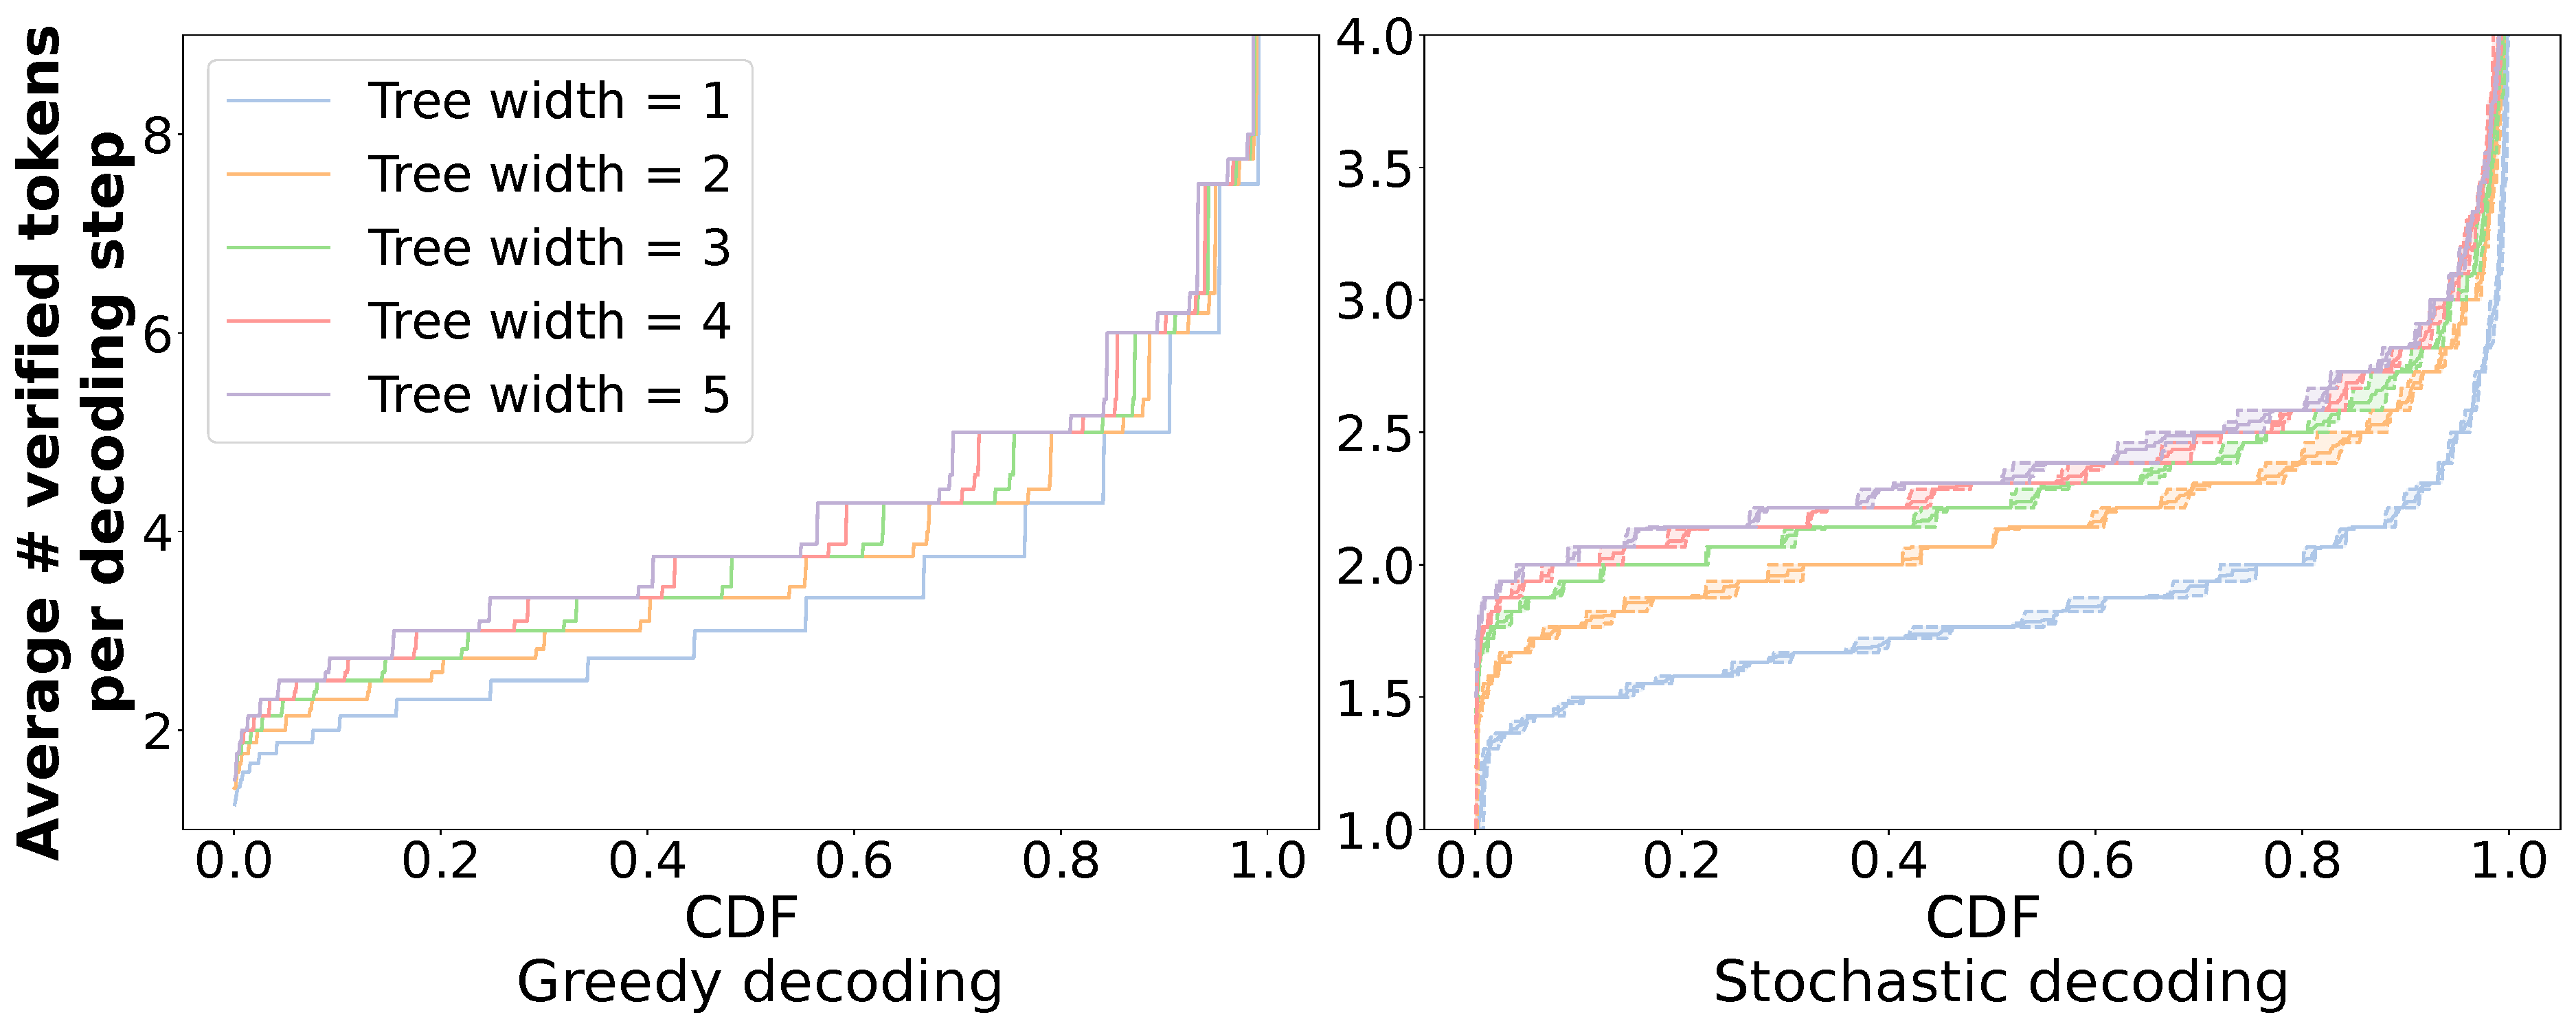
\includegraphics[width=\linewidth]{figs/alpaca_CDF.pdf}
    \caption{\rev{Comparing speculative performance of \sys with different token tree structures.}}
    % \caption{CDF figures of greedy sampling, stochastic sampling and greedy decoding. \ZJ{TODO: (1) increase font size for the y-axis title; (2) change the title to ``Average \# verified tokens per decoding step''; (3) add a ``='' between tree width and value}
    \label{fig:eval_cdf}
\end{figure}

% \if 0
% \begin{table}
% \begin{center}
% % \caption{Average number of tokens verified by \Sys in a decoding step.  We used \llama-7B as the LLM and used different numbers of collectively boost-tuned SSMs, all of which were derived from \llama-160M. The speculation length is 16 for all SSMs.}
% \caption{\ZX {Llama 68M Merge-based token tree (this caption and table label need to be modified).}}
% \footnotesize
% \label{tab:cbt-llama}
% \begin{tabular}{ccccccc}
% \toprule
% \# SSMs  & 1 & 2 & 3 & 4 & 5 \\ \midrule
% Alpaca       & 2.95     & 3.21    & 3.31     & 3.41     & \textbf{3.50}     \\
% CP           & 2.58     & 3.05    & 3.16     & 3.22     & \textbf{3.31}     \\
% WebQA        & 2.27     & 2.42    & 2.58     & 2.65     & \textbf{2.74}     \\
% CIP          & 2.73     & 3.12    & 3.24     & 3.41     & \textbf{3.52}     \\
% PIQA         & 2.18     & 2.44    & 2.54     & 2.62     & \textbf{2.73}         \\ \midrule
% %Avg        &1.34     & 1.39     & 1.60    & 1.67     & 1.73     & \textbf{1.79}      \\ \bottomrule
% \end{tabular}
% \end{center}
% \end{table}
% \fi


\begin{table}
\begin{center}
\caption{\rev{Average number of tokens verified by \sys in a decoding step. We use \llama-7B and \llama-68M as the LLM and SSM, and use different tree widths for constructing a token tree. The speculation length is 8.}}
%\caption{\textcolor{blue}{Llama 68M improved sample (this caption and table label need to be modified).}
%\footnotesize
\label{tab:cbt-llama}

\begin{tabular}{ll|ccccc}
\toprule
& & \multicolumn{5}{c}{{\bf Token tree width}} \\
& Dataset   & 1 & 2 & 3 & 4 & 5 \\ \midrule
\multirow{5}{*}{\rotatebox[origin=c]{90}{\parbox{2cm}{\bf \centering Greedy\\ decoding}}}
& Alpaca     & 2.95     & 3.07    & 3.21     & 3.33     & \textbf{3.43}     \\
& CP         & 2.58     & 3.24    & 3.46     & 3.59     & \textbf{3.69}     \\
& WebQA      & 2.27     & 2.69    & 2.86     & 2.98     & \textbf{3.07}     \\ 
& CIP        & 2.73     & 3.40    & 3.62     & 3.79     & \textbf{3.91}     \\
& PIQA       & 2.18     & 2.80    & 2.97     & 3.10     & \textbf{3.21}     \\  
\midrule
\multirow{5}{*}{\rotatebox[origin=c]{90}{\parbox{2cm}{\bf \centering Stochastic\\ decoding}}}
& Alpaca     & 1.79     & 2.11    & 2.26     & 2.32     & \textbf{2.38}     \\
& CP         & 1.69     & 1.99    & 2.15     & 2.23     & \textbf{2.28}     \\
& WebQA      & 1.64     & 1.93    & 2.08     & 2.15     & \textbf{2.21}     \\
& CIP        & 1.72     & 2.05    & 2.19     & 2.28     & \textbf{2.29}     \\
& PIQA       & 1.67     & 1.93    & 2.08     & 2.15     & \textbf{2.21}         \\ %\midrule
%Avg        &1.64     & 1.70     & 2.00    & 2.15     & 2.23     & \textbf{2.28}      \\ 
\bottomrule
\end{tabular}
\end{center}
\end{table}
%\begin{table}
\caption{Average number of tokens verified by \Sys in a decoding step. We used OPT-13B as the LLM and used different numbers of collectively boost-tuned SSMs, all of which were derived from OPT-125M. The speculation length is 16 for all SSMs.}
\label{tab:cbt-opt}
\begin{center}
\footnotesize
\begin{tabular}{cccccc}
\toprule
               \# SSMs             & 1 & 2 & 3 & 4 & 5 \\ \midrule
CIP & 3.00     & 3.39     & 3.52     & 3.58     & \textbf{3.74}     \\
CP           & 2.95     & 3.35     & 3.49     & 3.52     & \textbf{3.68}     \\
WebQA                      & 2.51     & 2.92     & 3.04     & 3.09     & \textbf{3.20}     \\
Alpaca               & 3.33     & 3.89     & 4.06     & 4.17     & \textbf{4.35}     \\
PIQA                        & 2.75     & 3.14     & 3.26     & 3.31     & \textbf{3.43}     \\ \midrule
Avg                         & 2.91     & 3.34     & 3.47     & 3.53     & \textbf{3.68}     \\ \bottomrule
\end{tabular}
\end{center}
\end{table}


\begin{figure}
    \centering
    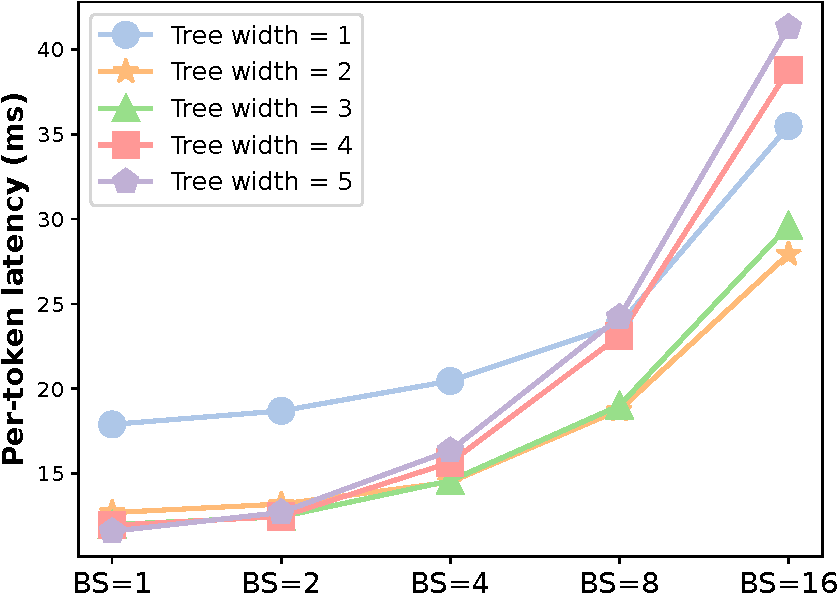
\includegraphics[scale=0.45]{figs/eval_tree_branches-crop.pdf}
    \caption{\rev{\Sys's end-to-end inference latency with different tree widths. We use \llama-7B and \llama-68M as the LLM and SSM.}}
    \label{fig:eval_tree_branches}
\end{figure}

\rev{A larger token tree width reduces the LLM decoding steps to process a request at the cost of increased verification overhead, since \sys must verify more tokens.
\Cref{fig:eval_tree_branches} compares the end-to-end inference latency of \sys using different tree widths.
%
For small batch sizes (i.e., BS = 1 and 2), using a large tree width can consistently reduce per-token latency, since \sys can leverage sparse GPU resources to verify more tokens in parallel while maintaining the same per-iteration latency.
%
For large batch sizes (i.e., BS $\geq 4$), using a large tree width increases the latency to verify a token tree due to less sparse GPU resources that can be leveraged by \sys, and a tree width of $2$ or $3$ achieves the best performance by striking a perfect balance between speculative performance and verification latency.}
%

\if 0
In this section, we evaluate the effectiveness of collective boost-tuning in terms of improving the average number of verified tokens in each LLM decoding step. 
%%%
%For both the OPT and \llama experiments, we fine-tuned four SSMs over the OpenWebText Corpus using collective boost-tuning on top of the pre-trained OPT-125M and \llama-160M models, which provides a collection of five SSMs (including the base SSM) in each experiment.
%%%
As shown in \Cref{tab:cbt-llama}, the average number of tokens verified by \Sys in each LLM decoding step increases consistently across all five datasets due to better alignment between the LLM and our tuned collection of SSMs.
%%%
More specifically, by using collectively boost-tuned SSMs, we have an overall improvement of $26.4\%$ and $22.6\%$ respectively, compared to using only a single pre-trained SSM.

We further study how different numbers of SSMs affect \Sys's inference latency. In this experiment, we use \llama-60B as the LLM and the five collectively boost-tuned \llama-160M models as the SSMs. \Sys uses tensor model parallelism to serve \llama-30B across 4 GPUs and uses data parallelism to serve SSMs on different GPUs. 
%%%
\Cref{fig:eval_ssms} shows the results.
%%%
\Sys's performance is insensitive to the number of SSMs for two reasons.
%%%
First, \Sys uses data parallelism to serve SSMs on different GPUs in parallel. 
As a result, adding more SSMs does not increase the speculation time and marginally increase the verification time (since \Sys needs to verify more tokens).
Second, as shown in \XM{\Cref{tab:cbt-opt}} and~\Cref{tab:cbt-llama}, the first several SSMs are critical to achieving high speculative performance and the average matching length increases slightly (i.e., from 3.27 to 3.58 and from 3.34 to 3.68 for OPT and \llama) as we introduce more SSMs. \XM{TODO: update}
\fi 

% \begin{figure}[H]
%     \centering
%     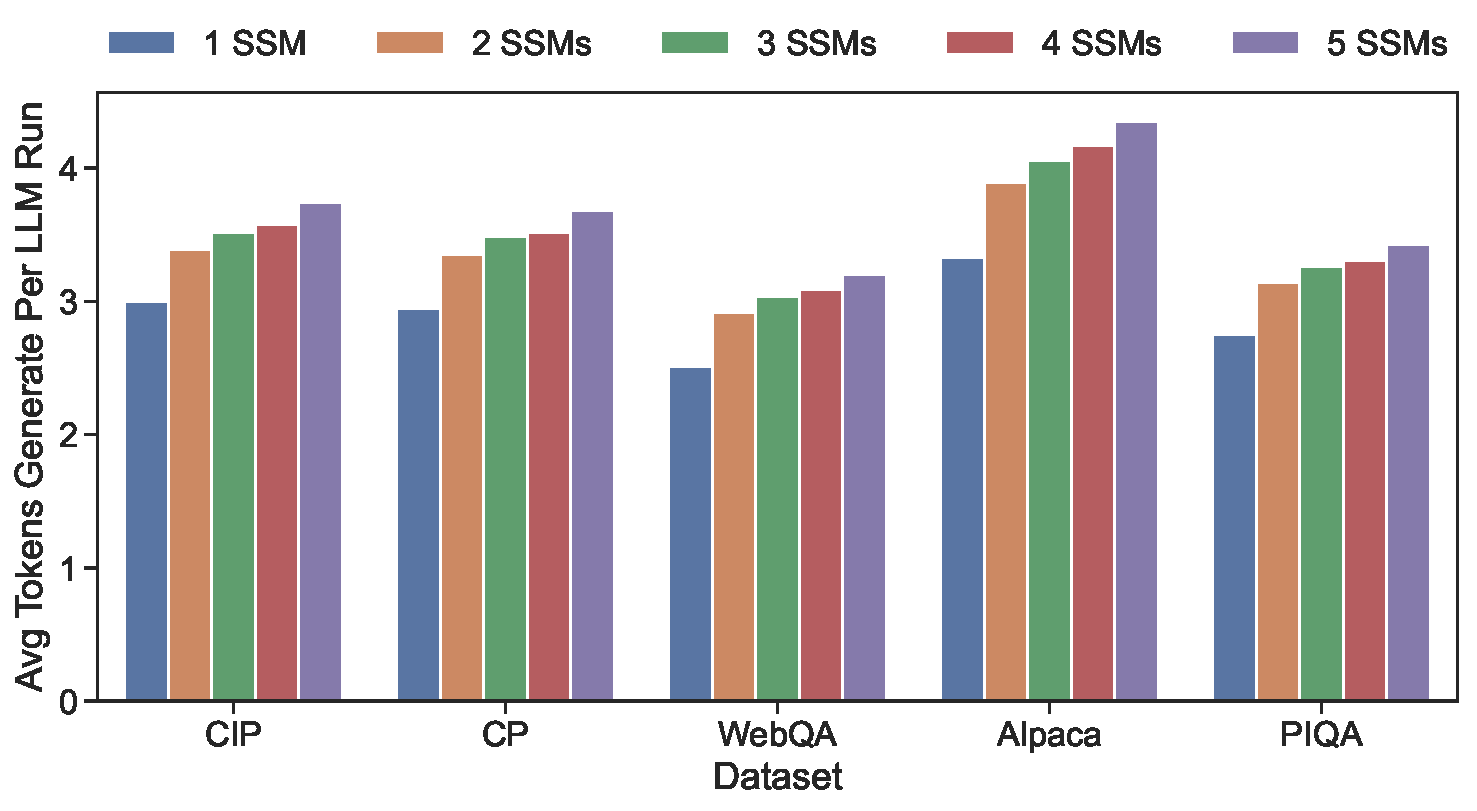
\includegraphics[width=\columnwidth]{figs/CBT-OPT.pdf}
%     \caption{Average number of tokens verified by \Sys in each LLM decoding step over five datasets. We use a fixed speculation length of 16 for all the SSMs in this experiment. We used OPT-13B as the LLM and used four SSMs boost-tuned from OPT-125M.}
%     \label{fig:CBT-OPT}
% \end{figure}


% \begin{figure}[H]
%     \centering
%     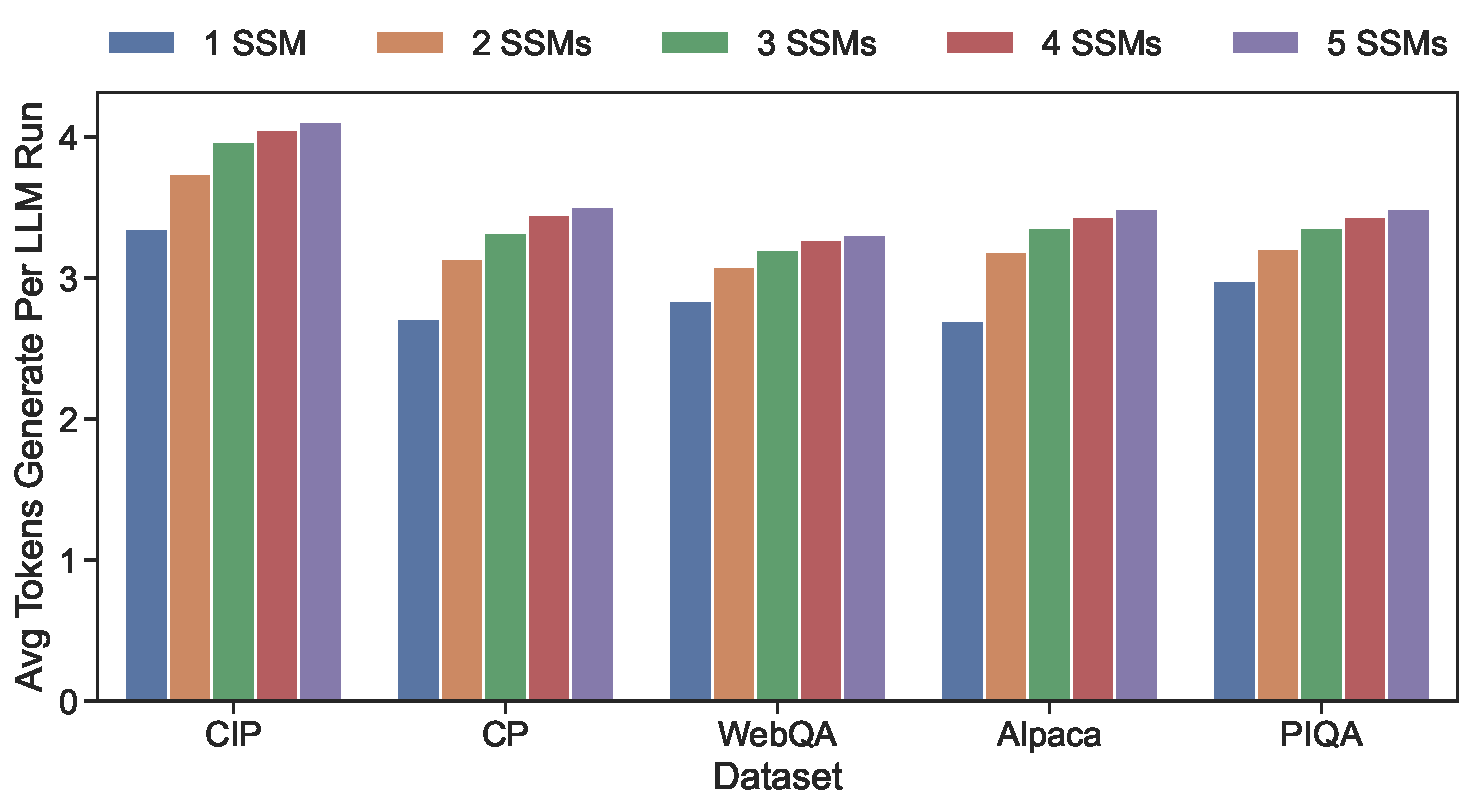
\includegraphics[width=\columnwidth]{figs/CBT-LLaMA.pdf}
%     \caption{Average number of tokens verified by \Sys in each LLM decoding step over five datasets. We use a fixed speculation length of 16 for all the SSMs in this experiment. We used \llama-7B as the LLM and used four SSMs boost-tuned from \llama-160M.}
%     \label{fig:CBT-LLaMA}
% \end{figure}

\if 0
\subsection{Learning-based Speculative Scheduler}
\label{subsec:eval_scheduler}
\ZJ{We will be removing the learning-based scheduler part right?}
For the learning-based speculative scheduler, we demonstrate some preliminary results on the matching length predictor in this section.
%%%
We use a three-layer MLP with a hidden feature size of 64 as our predictor.
%%%
We train the predictor on 200K samples over the OpenWebText corpus.
%%%
The labels are generated using OPT-13B as the LLM and OPT-125M as the SSM.
%%%
As shown in~\Cref{tab:lss-opt}, using the predictor can achieve similar LLM runs while reducing the SSM runs significantly due to dynamic speculation length. 
Nevertheless, there is still plenty of space to improve the predictor as the optimal SSM run would be the average matching length times the LLM run.

%%%
% \if 0
% \begin{table}[H]
% \caption{\XM{TODO: add a caption}}
% \label{tab:lss-opt}
% \begin{center}
% \begin{tabular}{ccccccccccc}
% \hline
%         & \multicolumn{2}{c}{CIP} & \multicolumn{2}{c}{CP} & \multicolumn{2}{c}{WebQA} & \multicolumn{2}{c}{Alpaca} & \multicolumn{2}{c}{PIQA} \\ \cline{2-11} 
%         & w/ oracle  & w/o oracle & w/ oracle & w/o oracle & w/ oracle   & w/o oracle  & w/ oracle   & w/o oracle   & w/ oracle  & w/o oracle  \\ \hline
% LLM Run & 8812       & 8449       & 3625      & 3462       & 12624       & 12080       & 11123       & 10684        & 12625      & 11560       \\
% SSM Run & 56401      & 135184     & 23172     & 55392      & 74953       & 193280      & 72863       & 170944       & 74548      & 184960      \\ \hline
% \end{tabular}
% \end{center}

% \end{table}

\begin{table}
\caption{The number of LLM runs and SSM runs with or without the presence of the matching length predictor. When there is no predictor, we use a fixed speculation length of 16 for all the SSMs in this experiment. LLM: OPT-13B, SSMs: OPT-125M}
\label{tab:lss-opt}
\begin{center}
\begin{tabular}{ccccc}
\toprule
       & \multicolumn{2}{c}{LLM run} & \multicolumn{2}{c}{SSM run} \\ \cmidrule{2-5} 
       & w/ predictor    & w/o predictor   & w/ predictor    & w/o predictor   \\ \midrule
CIP    & 8812         & 8449         & 56401        & 135184       \\
CP     & 3625         & 3462         & 23172        & 55392        \\
WebQA  & 12624        & 12080        & 74953        & 193280       \\
 Alpaca & 11123        & 10684        & 72863        & 170944       \\
PIQA   & 12625        & 11560        & 74548        & 184960       \\ \bottomrule
\end{tabular}
\end{center}
\end{table}
% \fi 
%%%
\fi

\subsection{\rev{Tree-based Parallel Decoding}}
\label{subsec:eval_tree_based_decoding}

\begin{figure}
    \centering
    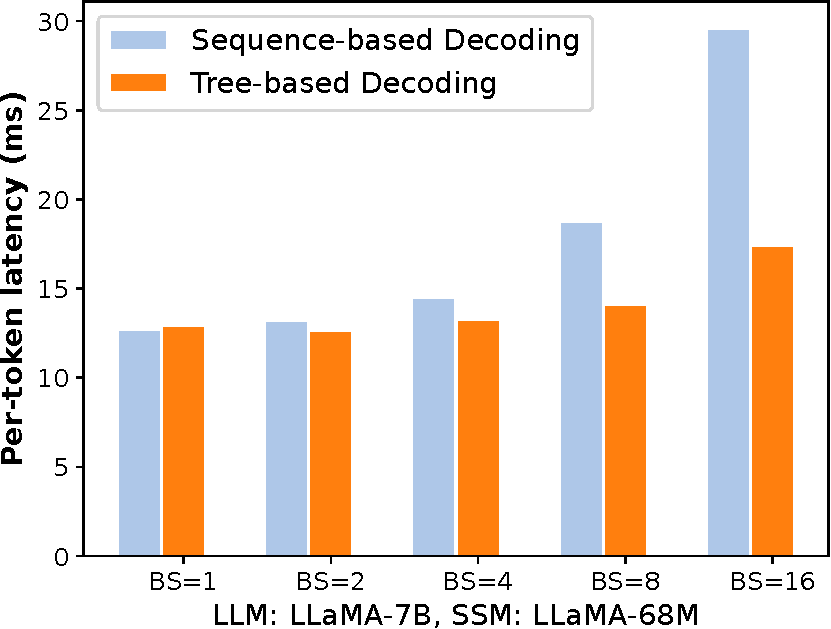
\includegraphics[scale=0.45]{figs/tree-based-decoding-crop.pdf}
    \caption{\rev{Comparing \Sys's tree-based parallel decoding with the sequence-based decoding mechanism employed by existing LLM inference systems.}}
    %\vspace{-4mm}
    \label{fig:eval_tree_based_decoding}
\end{figure}

\rev{We now evaluate the effectiveness of \sys's tree-based parallel decoding mechanism, which decodes all tokens of a token tree in parallel.
%
As a comparison, all existing LLM inference systems use sequence-based decoding, which requires decomposing a token tree into multiple sequences of tokens and processing these sequences using separate resources due to potential key-value cache conflicts (see \S\ref{subsec:optimization}).
%
% \Cref{fig:eval_tree_based_decoding} shows a comparison between the two methods. 
As shown in \Cref{fig:eval_tree_based_decoding}, \sys's tree-based parallel decoding achieves on-par performance as existing sequence-based decoding mechanism for small batch sizes and outperforms it by up to 1.8$\times$ for large batch sizes. The improvement is realized by (1) eliminating redundant attention computation for sequences with a shared prefix, and (2) fusing tree attention of all tokens in a single kernel through the topology-aware casual mask (see \S\ref{subsec:optimization}).}

\begin{table}
\begin{center}
\caption{\rev{Average number of tokens verified by \sys in a stochastic decoding step with different sampling algorithms. We use \llama-7B and \llama-68M as the LLM and SSM. Each token tree has a width of 5 and a depth of 8.}}
%\caption{\textcolor{blue}{Llama 68M improved sample (this caption and table label need to be modified).}
\label{tab:eval_msss}
\resizebox{\linewidth}{!}{%
\begin{tabular}{l|rrr}
\toprule
& {\bf Naive}  & {\bf Multi-Step} & {\bf Improvement} \\ 
& {\bf Sampling} & {\bf Spec. Sampling} & \\ \midrule
Alpaca     & 1.87     & 2.38    & 1.27$\times$\\
CP         & 1.80     & 2.28    & 1.26$\times$\\
WebQA      & 1.73     & 2.21    & 1.28$\times$\\ 
CIP        & 1.79     & 2.29    & 1.28$\times$\\
PIQA       & 1.73     & 2.21    & 1.28$\times$\\  
\bottomrule
\end{tabular}%
}
\end{center}
\end{table}

\subsection{\rev{Multi-Step Speculative Sampling}}
\label{subsec:eval_msss}


\rev{This section evaluates how our multi-step speculative sampling (MSS) and the \textproc{VerifyStochastic} algorithm improves the speculative performance of \sys when performing stochastic decoding.
%
We use naive sampling as a baseline where \sys directly samples the next token from the LLM and examines whether the sampled token is included in the speculated token tree (see \S\ref{subsec:verification}).
%
Since different sampling algorithms involve identical speculation and verification overheads, we focus on the average number of tokens that can be verified in each stochastic decoding step in this experiment.
%
\Cref{tab:eval_msss} shows the results. Compared to naive sampling, MSS can consistently improve the number of verified tokens by 1.2-1.3$\times$ on average across a variety of prompt datasets, while guaranteeing the same output distribution with the LLM.
%
}